\chapter{Evaluation}
\label{chap:Evaluation}

% TODO: talk about the methodology of the evaluation

In this chapter, the goal is to evaluate different use-cases for ML-based interpolation in the context of air temperature interpolation. In Chapter~\ref{chap:Machine Learning based Interpolation} the different models for ML-based interpolation were already introduced. Afterwards, the available data and features were introduced in Chapter~\ref{chap:preparations data sets}. In this chapter, the different models are compared with different data sets and features to test the feasability of two main use cases:

\begin{enumerate}
  \item Areal interpolation of air temperature (for a specific time step)
  \item Interpolation of air temperature for a specific location (over time)
\end{enumerate}

Next to these main uses cases we discuss in this work, the different regression models can be used in many other ways, primarily based on the features used during training. Some regression models could for example be used to predict future air temperature, however this is out of the scope of this work.

\subsubsection{Validation Methodology}
\label{sec:validation methodology}

In order to validate the different models, we use the following methodology:

\begin{itemize}
  \item The dataset is split into a training and test set. 70\% of the data is used for training and 30\% is completely withhold for testing. The training and test set are split randomly, but the same split is used for all models to ensure comparability.
  \item Additional reference stations are used where available to compare the interpolated values with reference values. Reference stations are stations that are operated by WMO standard, such as DWD stations. The reference stations are not used for training, but only for qualitative evaluation.
  \item The models are trained and evaluated using loss functions. The loss functions used in this work are: Mean Absolute Error (MAE), Mean Squared Error (MSE), Root Mean Squared Error (RMSE), and R2 Score and are shown for the evaluation.
\end{itemize}

Different loss functions have different advantages and disadvantages. For example the RSME is more robust against outliers while the MSE punishes bigger errors more. Depending on the use-case different loss functions can be better suited and should be evaluated.

\section{Areal Interpolation of Air Temperature}

- Reference of a traditional geostatistical method -> Kriging
  - smoothes out the area between points and fills in missing points
  - no extrapolation between the max-min of the 2 points because in between no information is known
  - some limitations such as that over time the mean does not change (not applicable for air temperature due to climate change?)

- in comparison, training a regressor with more features could potentionally give the model additonal information. Especially in the context of urban environments, information such as surface rougness levels, e.g. building and vegeation cover, sourced from remote sensing with good spatial coverage, could improve the prediction quality.

\subsection{Datasets for Evaluation}

As a first step for training and testing areal air temperature interpolation methods, we need to define the test area and the data we use for training. In this context, it could be interesting to compare different sensor network providers.
For this use-case we have several test areas that we could validate. To get an overview of the sensors left after QC for Sensor.Community, Table 

-> could also compare with Hamburg (closer to water, more wind)

- find locations that are:
  - somewhat near reference stations for comparison
  - high station density
  - interesting features (e.g. parks, water, ...)

- locations in Germany for Sensor.Community are:
  - Stuttgart (birthplace of Sensor.Community) with high station density + one reference station somewhat close
  - Hamburg with lower sensor density, but 2 reference stations (interesting to see changes between those over realtively short distances) and close to water/river (Elbe)
  - other candidates (but with way fewer sensor and no reference stations): Cologne, Munich, Freiburg (interesting that they have an airport but no reference station), Lüneburg
  - interesting to note, that Berlin did not have any sensor stations that passed the QC step\\

\begin{figure}[ht]
    \centering
    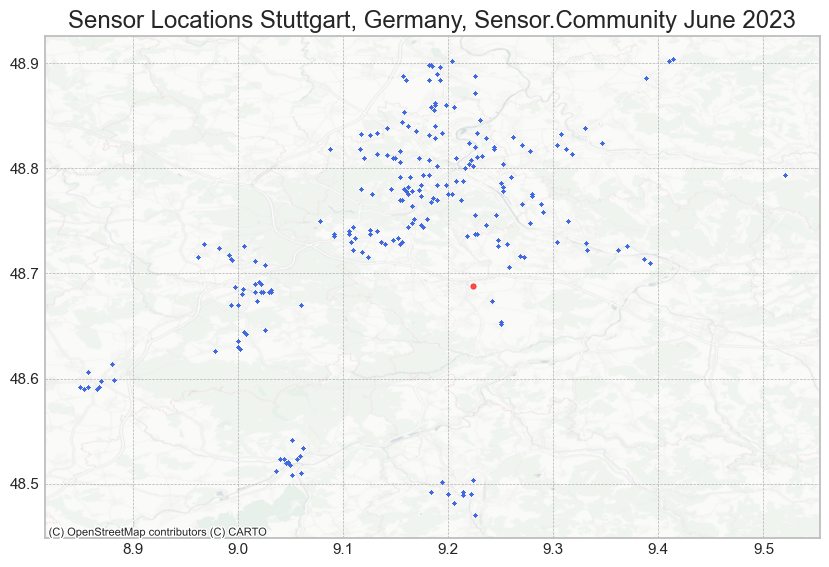
\includegraphics[width=1\textwidth]{images/sensor_community_locations_stuttgart_after_qc_june_23.png}
    \caption{Locations for Sensor.Community around Stuttgart, Germany, June 2023}
    \label{fig:qc sensor community stuttgart june 23}

    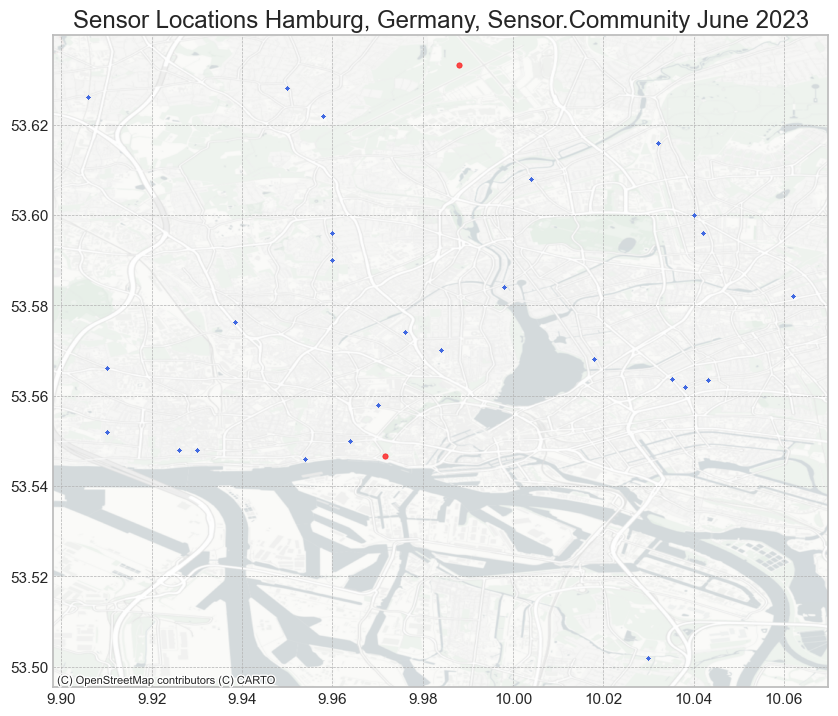
\includegraphics[width=1\textwidth]{images/sensor_community_locations_hamburg_after_qc_june_23.png}
    \caption{Locations for Sensor.Community in Hamburg, Germany, June 2023}
    \label{fig:qc sensor community hamburg june 23}
\end{figure}

- we choose stations from Stuttgart and Hamburg for the evaluation
-> identify stations with high mean daily temperature difference to reference station (to see if they are in a heat island)

\subsubsection{Stuttgart}

Station Locations:\\

\begin{figure}[ht]
    \centering
    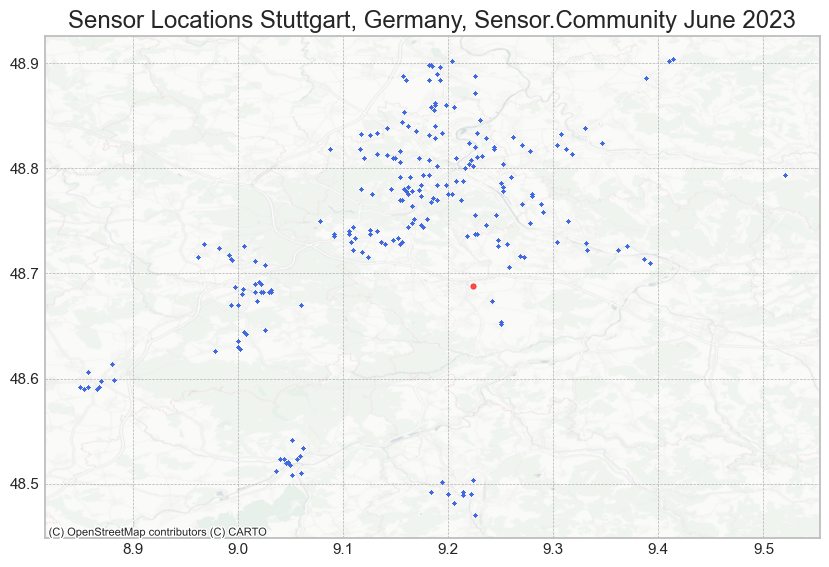
\includegraphics[width=1\textwidth]{images/sensor_community_locations_stuttgart_after_qc_june_23.png}
    \caption{Locations for Sensor.Community around Stuttgart, Germany, June 2023}
\end{figure}

DWD Reference location: 48.6883;9.2235 -> DWD id: 4931, Daily Max, Mean and Min values for June 2023\\

\begin{figure}[ht]
    \centering
    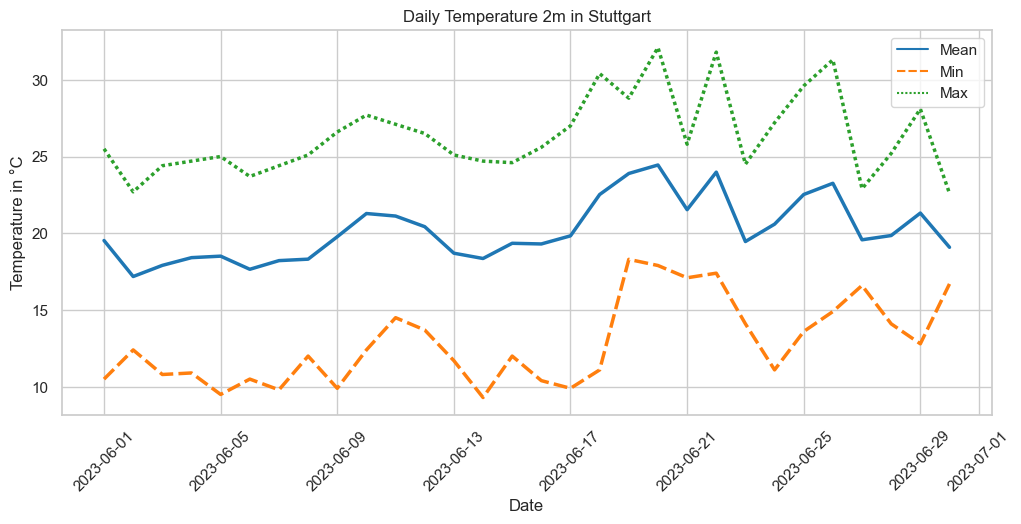
\includegraphics[width=1\textwidth]{images/dwd_stuttgart_june_23_tair_max_mean_min.png}
    \caption{Daily Mean, Max, and Min Air Temperature at 2m in Stuttgart, Germany, June 2023, DWD Station 4931}
    \label{fig:dwd mean max min stuttgart june 23}
\end{figure}

\subsubsection{Hamburg}

Todo: add Hamburg station locations\\

\section{Model Evaluation}

Choose one model that performs the best

\section{Variable Importance}

\subsection{Geostatical Interpolation Comparison}
In order to evaluate the performance of the ML model, we need to first get a better understanding of the interpolation quality of existing interpolation techniques. Next to simpler deterministic interpolation methods, such as inverse weight distance (IWD) or k-nearest neighbours (KNN) that are easy and performant, but struggle to capture more complex interdependencies, there are also more complex methods available. The most common geostatistical method for interpolation is Krigin, which is based on a gaussian process and uses a covariance function to model the spatial correlation between data points. The covariance function is a measure of the similarity between two data points, which is used to calculate the weight of the data point in the interpolation process. There are different types of Krigin methods available, each suited for different use cases, including:

\begin{enumerate}
    \item Simple Krigin: the simplest form of Krigin, that assumes that the mean of the measured values is known and constant
    \item Ordinary Krigin: same as Simple Krigin, but the mean is an unknown constant
    \item Universal Krigin: instead of assuming a constant mean, the mean is modeled as a deterministic function
    \item Indicator Krigin: same as Ordinary Krigin, but for categorical data
    \item Propability Krigin: same as Indicator Krigin, but assumes two types of random errors that can are each auto-correlated and cross-correlated to each other
    \item Disjunctive Krigin: same as Ordinary Krigin, but tries to improve the prediction quality by using an unknown constant and approximating an arbitrary function. It requires the bivariate normality assumption and is difficult to verify and solutions might be mathematically and computationally complicated
    \item Cokrigin: offers methods for the previous Krigin methods, but uses information on several variable types. This could improve the prediction quality, but might increase the variance of the prediction, as more much more estimation is required
\end{enumerate}

In the context of geostatistical analysis, there are different types of Krigin methods available that combine the aforementioned methods with other techniques, such as regression analysis. The following list is the geostaticial methods offered by ArcGIS Pro as part of the Geostatical Analyst toolbox~\footnote{\url{https://pro.arcgis.com/en/pro-app/latest/tool-reference/geostatistical-analyst/an-overview-of-the-geostatistical-analyst-toolbox.htm}}:

% TODO: add more details for each method
\begin{enumerate}
    \item Empirical Bayesian Krigin (EBK)
    \item Empircal Bayesian Krigin 3D (EBK3D)
    \item EBK Regression Prediction (EBKRP): Empirical Bayesian Kriging with regression prediction
    \item Global Polynominal Interpolation
    \item Kernel Interpolation with Barriers
    \item Moving Window Krigin
    \item Radial Basis Function
\end{enumerate}

In the scope of this work, we unfortunately cannot compare all of these methods with each other and therefore need to focus on a subset of methods. EBK and EBKRP are one of the most commonly used methods for temperature interpolation (cite). According to \cite{njoku2023effects}, EBKRP continously outperforms EBK in different weather station density scenarios, therefore we will use EBKRP as a baseline for our comparison.\\
In the following, the machine learning fundamentals for this work are explained and the different ML regression model types are introduced.

\section{Interpolation of Air Temperature for a Specific Location}


TODO
First compare only air temperature for stations that are near a reference station and have enough buddies for sensor community
- only for june 2023 from sensor community, not january as heat islands are not as important in winter (which depends on the context ofc if the goal is f.e. to save heating costs, could be a factor)

Steps in the evaluation:
- find sensor community stations near reference stations that passed m5 QC step
- Compare different interpolation approaches
  - linear, forests, KNN, NNetwork
  - with different amounts of data available (99\% -> 1\%) and see how RSME evolves

1. Data Collection and rough analysis
  1.1. Get data from Sensor.Community
  1.2. Get data from DWD
  1.3. Get data from satellites via Google Earth Engine
  1.4. Get data from Netatmo (Hamburg, try to get Stuttgart as reference with historical data via API)
2. QC steps (TA first)
  2.1. Try to remove indoor stations and stations with irregular data
  2.2. Remove stations based on buddy check (removes a lot of sensor community stations due to lower density)
  2.3. Reference station has high quality data already, but can be used as a reference (interesting the comparison from 2m TA to 5cm TA)
  2.4. Discuss QA for other parameters (Humidity, Pressure etc.)
3. Comparison of models
  3.1. Simple models with only coordinates as input features and TA as target feature
  3.2. Add additional features (land coverage (NDVI, EVI)) and see how they improve the model
    3.2.1. For land coverage etc.\ compare different satellites and resolutions
    3.2.2. For coordinates/distances, compare different ways of calculating distances or modelling them in the model
    3.2.3. Compare influence of normalization
  3.3. Try to create a more complex NN model to show capabilities of NNs and try out LSTM for time series
  3.4. Compare different loss functions and metrics (MSE, MAE, RMSE)
  3.5. Choose final candidate that seems the most promissing and compare with reference approach
4. Comparison with refrence approaches
  4.1. Compare with simple Ordinary Kriging approach (with different kernels)
  4.2. Discuss problem of not being able to extrapolate




Steps:
- deterministic approaches
  - "naive" approach with nearest neighbor -> show high error rate
- probabilistic approaches
  - reference approach with geostatical methods (ordinary kriging, empirical bayesian kriging, EBK with regression) -> still high error rate, especially with lower density of weather stations/bad support for irregularly spaced data
    - ordinary krigin:
        - temperature semivariogram first
        - add additional features (e.g. soil temperature, land coverage, sky view factor, ...) as semivariograms and use cokrigin to combine them
    - empirical bayesian kriging:
        - not implemented out of the box (pykrige)

  - semivariogram: https://pro.arcgis.com/en/pro-app/latest/help/analysis/geostatistical-analyst/understanding-a-semivariogram-the-range-sill-and-nugget.htm

- deep learning approach with neural networks -> itteratively improve model by adding additional features, compare with reference approach



\section{Model Evaluation}

TODO

\subsection{Model Validity}

% TODO
Use 70\% of data for training, 30\% for test. cross-validation

\section{Variable Importance}

\section{Uncertainty Analysis}

measurement uncertainty, contextual uncertainty, prediction uncertainty

% Overall steps

1. Data Collection and rough analysis
  1.1. Get data from Sensor.Community
  1.2. Get data from DWD
  1.3. Get data from satellites via Google Earth Engine
  1.4. Get data from Netatmo (Hamburg, try to get Stuttgart as reference with historical data via API)
2. QC steps (TA first)
  2.1. Try to remove indoor stations and stations with irregular data
  2.2. Remove stations based on buddy check (removes a lot of sensor community stations due to lower density)
  2.3. Reference station has high quality data already, but can be used as a reference (interesting the comparison from 2m TA to 5cm TA)
  2.4. Discuss QA for other parameters (Humidity, Pressure etc.)
3. Comparison of models
  3.1. Simple models with only coordinates as input features and TA as target feature
  3.2. Add additional features (land coverage (NDVI, EVI)) and see how they improve the model
    3.2.1. For land coverage etc.\ compare different satellites and resolutions
    3.2.2. For coordinates/distances, compare different ways of calculating distances or modelling them in the model
    3.2.3. Compare influence of normalization
  3.3. Try to create a more complex NN model to show capabilities of NNs and try out LSTM for time series
  3.4. Choose final candidate that seems the most promissing and compare with reference approach
4. Comparison with refrence approaches
  4.1. Compare with simple Ordinary Kriging approach (with different kernels)
  4.2. Discuss problem of not being able to extrapolate